\begin{figure}[H]
\centering
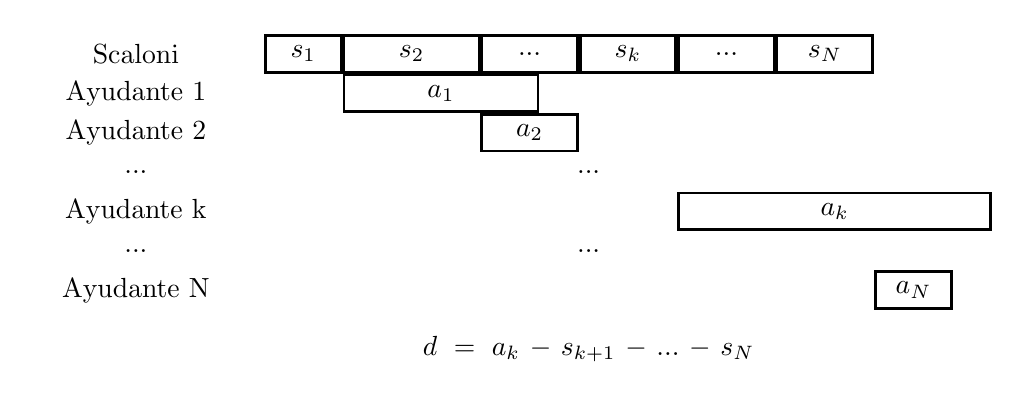
\begin{tikzpicture}
	% Paths, nodes and wires:
	\node[shape=rectangle, draw, line width=1pt, minimum width=0.965cm, minimum height=0.465cm] at (3.5, 5.75){} node[anchor=center, align=center, text width=0.577cm, inner sep=6pt] at (3.5, 5.75){$s_1$};
	\node[shape=rectangle, draw, line width=1pt, minimum width=1.715cm, minimum height=0.465cm] at (4.875, 5.75){} node[anchor=center, align=center, text width=1.327cm, inner sep=6pt] at (4.875, 5.75){$s_2$};
	\node[shape=rectangle, draw, line width=1pt, minimum width=2.465cm, minimum height=0.465cm] at (5.25, 5.25){} node[anchor=center, align=center, text width=2.077cm, inner sep=6pt] at (5.25, 5.25){$a_1$};
	\node[shape=rectangle, draw, line width=1pt, minimum width=1.215cm, minimum height=0.465cm] at (6.375, 4.75){} node[anchor=center, align=center, text width=0.827cm, inner sep=6pt] at (6.375, 4.75){$a_2$};
	\node[shape=rectangle, draw, line width=1pt, minimum width=1.215cm, minimum height=0.465cm] at (6.375, 5.75){} node[anchor=center, align=center, text width=0.827cm, inner sep=6pt] at (6.375, 5.75){...};
	\node[shape=rectangle, draw, line width=1pt, minimum width=1.215cm, minimum height=0.465cm] at (7.625, 5.75){} node[anchor=center, align=center, text width=0.827cm, inner sep=6pt] at (7.625, 5.75){$s_k$};
	\node[shape=rectangle, draw, line width=1pt, minimum width=3.965cm, minimum height=0.465cm] at (10.25, 3.75){} node[anchor=center, align=center, text width=3.577cm, inner sep=6pt] at (10.25, 3.75){$a_k$};
	\node[shape=rectangle, draw, line width=1pt, minimum width=1.215cm, minimum height=0.465cm] at (8.875, 5.75){} node[anchor=center, align=center, text width=0.827cm, inner sep=6pt] at (8.875, 5.75){...};
	\node[shape=rectangle, draw, line width=1pt, minimum width=1.215cm, minimum height=0.465cm] at (10.125, 5.75){} node[anchor=center, align=center, text width=0.827cm, inner sep=6pt] at (10.125, 5.75){$s_N$};
	\node[shape=rectangle, draw, line width=1pt, minimum width=0.965cm, minimum height=0.465cm] at (11.25, 2.75){} node[anchor=center, align=center, text width=0.577cm, inner sep=6pt] at (11.25, 2.75){$a_N$};
	\node[shape=rectangle, minimum width=2.715cm, minimum height=0.465cm] at (1.375, 5.75){} node[anchor=center, align=center, text width=2.327cm, inner sep=6pt] at (1.375, 5.75){Scaloni};
	\node[shape=rectangle, minimum width=2.715cm, minimum height=0.465cm] at (1.375, 5.25){} node[anchor=center, align=center, text width=2.327cm, inner sep=6pt] at (1.375, 5.25){Ayudante 1};
	\node[shape=rectangle, minimum width=2.715cm, minimum height=0.465cm] at (1.375, 4.75){} node[anchor=center, align=center, text width=2.327cm, inner sep=6pt] at (1.375, 4.75){Ayudante 2};
	\node[shape=rectangle, minimum width=2.715cm, minimum height=0.465cm] at (1.375, 3.75){} node[anchor=center, align=center, text width=2.327cm, inner sep=6pt] at (1.375, 3.75){Ayudante k};
	\node[shape=rectangle, minimum width=2.715cm, minimum height=0.465cm] at (1.375, 2.75){} node[anchor=center, align=center, text width=2.327cm, inner sep=6pt] at (1.375, 2.75){Ayudante N};
	\node[shape=rectangle, minimum width=2.715cm, minimum height=0.465cm] at (1.375, 4.25){} node[anchor=center, align=center, text width=2.327cm, inner sep=6pt] at (1.375, 4.25){...};
	\node[shape=rectangle, minimum width=2.715cm, minimum height=0.465cm] at (1.375, 3.25){} node[anchor=center, align=center, text width=2.327cm, inner sep=6pt] at (1.375, 3.25){...};
	\node[shape=rectangle, minimum width=2.715cm, minimum height=0.465cm] at (7.125, 4.25){} node[anchor=center, align=center, text width=2.327cm, inner sep=6pt] at (7.125, 4.25){...};
	\node[shape=rectangle, minimum width=2.715cm, minimum height=0.465cm] at (7.125, 3.25){} node[anchor=center, align=center, text width=2.327cm, inner sep=6pt] at (7.125, 3.25){...};
	\node[shape=rectangle, minimum width=6.215cm, minimum height=0.465cm] at (7.125, 2){} node[anchor=center, align=center, text width=5.827cm, inner sep=6pt] at (7.125, 2){$d = a_k- s_{k+1} -...-s_{N}$};
\end{tikzpicture}
    \caption{Análisis de tiempos para N rivales.}
    \label{fig:escenarios_posibles}
\end{figure}